\documentclass[11pt,a4paper]{article}

% ── Compilar con: tectonic x5_informe.tex  (motor XeTeX, UTF-8 nativo) ──
% Respaldo de contexto (todo lo rescatado de X5_otros/ y X5/): contexto_x5.md
\usepackage{fontspec}
\usepackage{amsmath,amssymb}
\usepackage[margin=2.2cm]{geometry}
\usepackage{xcolor}
\usepackage{booktabs}
\usepackage{tabularx}
\usepackage{enumitem}
\usepackage{underscore}
\usepackage{titlesec}
\usepackage{caption}
\usepackage{float}
\usepackage{pgfplots}
\pgfplotsset{compat=1.18}
\usetikzlibrary{arrows.meta,positioning,calc}
\usepackage[hidelinks]{hyperref}

% ── Colores (mismos que x5_v3_informe.tex y x5_alt_v2_opus.tex) ──
\definecolor{cazul}{HTML}{2C5F8A}
\definecolor{cverde}{HTML}{2E8B57}
\definecolor{cnaranja}{HTML}{C1660A}
\definecolor{cmorado}{HTML}{6B4FA0}
\definecolor{cgris}{HTML}{5B6770}
\definecolor{crojo}{HTML}{B3261E}
\definecolor{serieA}{HTML}{2A78D6}
\definecolor{serieB}{HTML}{EB6834}
\definecolor{tinta2}{HTML}{52514E}

\setlist{itemsep=2pt, topsep=4pt}
\emergencystretch=3em
\captionsetup{font=small, labelfont=bf, labelsep=period}
\renewcommand{\contentsname}{Índice}
\renewcommand{\tablename}{Tabla}
\renewcommand{\figurename}{Figura}
\titleformat{\section}{\normalfont\Large\bfseries\color{cazul}}{\thesection}{0.6em}{}
\titleformat{\subsection}{\normalfont\large\bfseries\color{cazul}}{\thesubsection}{0.6em}{}
\titlespacing*{\section}{0pt}{2.2ex plus 1ex minus .2ex}{1.0ex plus .2ex}
\titlespacing*{\subsection}{0pt}{1.8ex plus 1ex minus .2ex}{0.8ex plus .2ex}

\newcommand{\code}[1]{\texttt{\small #1}}
\newcommand{\mn}[1]{$-$#1}

\newenvironment{caja}[1]{%
  \par\medskip\noindent
  \begin{tabular}{@{}p{0.4em}@{\hspace{8pt}}p{\dimexpr\linewidth-2em\relax}@{}}
  \textcolor{#1}{\rule{3pt}{1.1em}} &
}{\end{tabular}\par\medskip}
\newenvironment{nota}{\begin{caja}{cnaranja}}{\end{caja}}
\newenvironment{clave}{\begin{caja}{cmorado}}{\end{caja}}
\newenvironment{advertencia}{\begin{caja}{crojo}}{\end{caja}}

\pgfplotsset{
  estilo/.style={
    axis line style={tinta2!60}, tick style={tinta2!60},
    major grid style={gray!18}, tick label style={font=\footnotesize, color=black},
    label style={font=\footnotesize, color=tinta2},
    legend style={font=\footnotesize, draw=none, fill=none},
    legend cell align=left,
    /pgf/number format/use comma, /pgf/number format/1000 sep={.},
  },
}

\title{\vspace{-1.6cm}\textbf{X5 — empezar de nuevo con un instrumento que funcione}\\[6pt]
  \large Qué dejó el X5 anterior, qué se rescata y un plan paso a paso para lograr parámetros\\
  dinámicos que le ganen a la mejor configuración estática\\[4pt]
  \normalsize\color{cgris} Revisión completa de \code{X5\_otros/} y \code{X5/} (código, notebooks, documentos, decisiones y datos)}
\author{Claude (Sonnet 5.5) para Mauricio Valdivia}
\date{22 de noviembre de 2026}

\begin{document}
\maketitle
\vspace{-0.6cm}

% ════════════════════════════════════════════════════════════════════
\section*{Resumen ejecutivo}

Me pediste revisar todo el X5 anterior y el trabajo ya hecho en \code{X5/}, proponer un informe nuevo,
un documento de contexto para no volver a abrir \code{X5\_otros/} y un plan paso a paso, con pruebas,
bifurcaciones y replanteos si hacen falta, siempre buscando la solución más simple. Leí los 23 archivos de
código (ocho de ellos con 96 pruebas), los siete notebooks (texto y resultados), los documentos y las
revisiones previas, las decisiones de junio a noviembre y el inventario de los 615~MB de datos. Todo lo rescatable quedó en
\code{X5/contexto\_x5.md}; este informe es el diagnóstico y el plan.

\begin{enumerate}[leftmargin=1.4em]
  \item \textbf{La misión sigue siendo buena; lo que falló fue el instrumento.} Se intentó aprender unas
        30 perillas a la vez con un banco de pruebas que no detecta el efecto de ninguna: el ruido de la
        semana domina, el backtest de cada ventana no mide a X0 (la búsqueda de soportes se corta por
        tiempo y entrega casi una escalera pareja) y la cuenta nueva de cada semana no ve las pérdidas
        encadenadas.
  \item \textbf{Aparecieron hallazgos que el informe del 21 de noviembre no tenía.} Los parámetros en
        dólares significan cosas distintas entre activos y años (la pérdida máxima nunca se habría activado
        en tres de siete activos); las ventanas están en velas y no en tiempo (en acciones «30 días» son 72);
        el «\code{N} dinámico» era sobre todo un \code{N} más bajo; la calibración de Q4 es circular;
        y, lo más urgente, \textbf{\code{X4\_backtester.py} hoy no se puede ni importar} porque depende de un
        archivo que se movió a \code{X5\_otros/}.
  \item \textbf{Tus tres decisiones de hoy fijan el rumbo.} El criterio es un híbrido: el retorno total
        de la cuenta continua es la vara final, y la ganancia semanal pareada es el filtro rápido. X5 solo
        vale si hay dinamismo (la mejor estática es el rival a vencer, no una meta). Y el Mac queda casi
        dedicado (30 o más horas de cómputo por semana).
  \item \textbf{Propuesta: un embudo para medir y una escalera para subir.} El embudo de tres niveles
        mide barato (segundos) y confirma caro (horas) solo a los finalistas. La escalera del dinamismo
        parte de la mejor estática y sube un peldaño solo si el anterior no basta: primero parámetros en
        unidades de volatilidad (un número), luego modulación, regímenes, freno de exposición y recién al
        final los parámetros de búsqueda o un modelo aprendido. Cada peldaño tiene su hipótesis, su
        criterio de éxito pre-registrado y su criterio de abandono.
  \item \textbf{El plan tiene siete fases y cuatro bifurcaciones} (§\ref{sec:plan}). Cabe en unas 12
        semanas con tu cómputo, parte por reparar X4 y archivar lo rescatado, y si la escalera se agota sin
        encontrar dinamismo no se cierra X5 solo: se abren replanteos ya preparados (§\ref{sec:rescate}).
\end{enumerate}

\begin{clave}
\textbf{En una frase}: antes de enseñarle a los parámetros cómo moverse, hay que poder medir en segundos,
en las mismas semanas, con riesgo y contra la mejor configuración fija, si moverlos mejora algo. Todo lo
demás (variables, curvas, modelos) viene después y solo si ese instrumento dice que vale la pena.
\end{clave}

\begin{nota}
\textbf{Qué no hice}: no corrí backtests nuevos ni modifiqué código de producción. Solo escribí documentos y
actualicé \code{todos.md} y \code{CLAUDE.md}. X4 se arregla junto con el motor de X5 (Fases 0b y 1, §\ref{sec:f0}),
con un diseño conjunto que tú apruebas antes de que se toque código.
\end{nota}

% ════════════════════════════════════════════════════════════════════
\section{Dónde estamos: la historia en una página}

\begin{figure}[H]
\centering
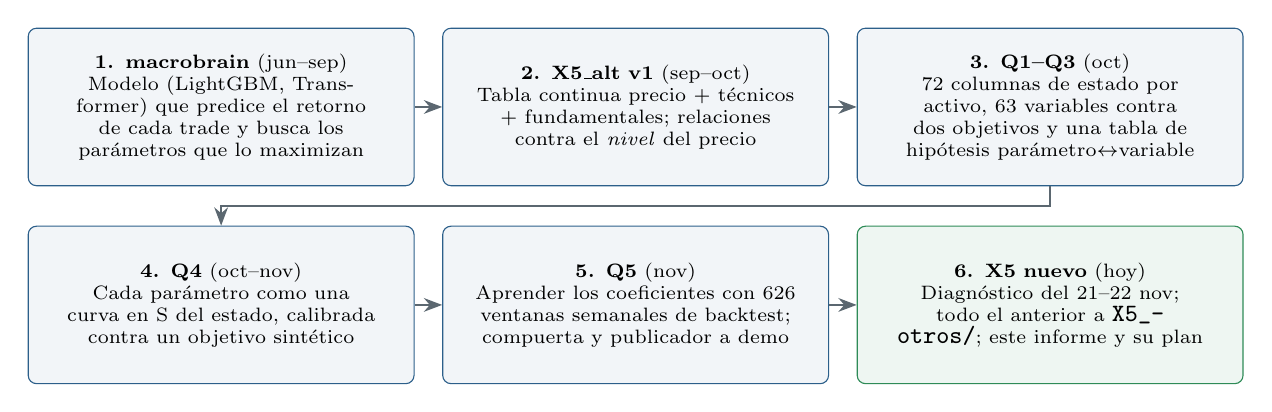
\begin{tikzpicture}[
  etapa/.style={draw=cazul, rounded corners=3pt, fill=cazul!6, minimum width=4.9cm, text width=4.6cm, minimum height=2.0cm,
                align=center, font=\scriptsize, inner sep=3pt},
  hoy/.style={etapa, draw=cverde, fill=cverde!8},
  flecha/.style={-{Stealth}, color=cgris, thick}]
\node[etapa] (e1) {\textbf{1. macrobrain} (jun--sep)\\Modelo (LightGBM, Transformer) que predice el retorno de cada trade y busca los parámetros que lo maximizan};
\node[etapa, right=0.35cm of e1] (e2) {\textbf{2. X5\_alt v1} (sep--oct)\\Tabla continua precio + técnicos + fundamentales; relaciones contra el \emph{nivel} del precio};
\node[etapa, right=0.35cm of e2] (e3) {\textbf{3. Q1--Q3} (oct)\\72 columnas de estado por activo, 63 variables contra dos objetivos y una tabla de hipótesis parámetro$\leftrightarrow$variable};
\node[etapa, below=0.5cm of e1] (e4) {\textbf{4. Q4} (oct--nov)\\Cada parámetro como una curva en S del estado, calibrada contra un objetivo sintético};
\node[etapa, right=0.35cm of e4] (e5) {\textbf{5. Q5} (nov)\\Aprender los coeficientes con 626 ventanas semanales de backtest; compuerta y publicador a demo};
\node[hoy, right=0.35cm of e5] (e6) {\textbf{6. X5 nuevo} (hoy)\\Diagnóstico del 21--22 nov; todo el anterior a \code{X5\_otros/}; este informe y su plan};
\draw[flecha] (e1)--(e2); \draw[flecha] (e2)--(e3); \draw[flecha] (e3.south) -- ++(0,-0.25) -| (e4.north);
\draw[flecha] (e4)--(e5); \draw[flecha] (e5)--(e6);
\end{tikzpicture}
\caption{Las etapas del X5 hasta hoy. Cada una nace de lo que la anterior dejó sin resolver.}
\end{figure}

Lo que cada etapa dejó \textbf{sin cerrar}: el macrobrain nunca se validó económicamente; Q1--Q3 dejó hipótesis
y no evidencia; Q4 dejó curvas que ajustan «por construcción»; Q5 construyó una infraestructura valiosa
(ventanas, cuenta de 3.000~USD, tope de Órdenes Abiertas, 627 conjuntos de soportes guardados) pero su
aprendizaje no encontró señal. El 21 de noviembre concluiste que la metodología de X5\_alt\_v2 no iba por
buen camino y el X5 anterior se movió a \code{X5\_otros/}, un directorio que \textbf{existe solo en tu Mac} (sin
copia en GitHub): conviene respaldarlo antes de moverlo o borrarlo (§\ref{sec:decisiones}).

\begin{table}[H]
\centering\small
\begin{tabularx}{\linewidth}{p{6.6cm}Xr}
\toprule
Qué se construyó & Estado & Tamaño \\
\midrule
Código del macrobrain y su recolección con X4 & obsoleto; acoplado a X4 (§\ref{sec:f0}) & 3 archivos \\
Variables de estado causales (\code{x5\_alt\_variables.py}) & rescatable con ajustes (§\ref{sec:variables}) & 250 líneas, 4 pruebas \\
Ventana semanal y orquestador (\code{X4\_bckt\_ventanas.py}, \code{X4S\_…}) & núcleo rescatable & 1.400 líneas, 44 pruebas \\
Aprendizaje RLM + gradiente, publicador, registro de demo & se descarta (patrón reutilizable) & 700 líneas, 34 pruebas \\
Notebooks Q1--Q4, P1, P2 y exploratorio & se descartan; el estándar de reporte vive en \code{docs/context/} & 17~MB \\
Datos de ventanas, soportes y cuentas (\code{q5/}) & \textbf{insustituible} sin ~100~h de cómputo & 104~MB \\
\bottomrule
\end{tabularx}
\caption{Inventario resumido (el veredicto por pieza está en el Anexo~A y, con argumentos, en \code{contexto\_x5.md} §6).}
\end{table}

% ════════════════════════════════════════════════════════════════════
\section{Lo que aprendimos}

Cada hallazgo sigue el mismo orden: qué vimos, por qué importa y qué hacemos con eso. Las cifras de ventanas
son las de hoy (320 de BTCUSD y 306 de TSLA); el análisis del 21 de noviembre usó 287 y 273 y no cambia.

\subsection{El ruido de la semana tapa la señal, y la forma de verla es comparar en pares}
\textbf{Qué vimos.} Dos configuraciones distintas corridas sobre la misma semana se parecen mucho (correlación
de 0,60 a 0,97), pero los dos controles del modelo (retorno medio y volatilidad de la semana) capturan solo
el 14~\% de lo que varía el resultado. Lo común entre configuraciones no son dos números resumen: es \emph{el camino
completo del precio} (cuántas veces cruza los soportes, cuándo cae, cuánto rebota). La única forma de restar
ese efecto es comparar ambas configuraciones \emph{en la misma semana}, con la misma semilla.

\textbf{Por qué importa.} Restar el efecto de la semana reduce la varianza entre 1,5 y 17 veces, que equivale a
tener ese número de veces más semanas. Aun así, para detectar una mejora de 25~USD por semana en BTCUSD harían
falta unas 1.200 semanas pareadas; la historia entera tiene 240 (Figura~\ref{fig:potencia}). En TSLA, con menos
dispersión, bastan 71. Además el resultado tiene colas muy pesadas (curtosis de 26 en BTCUSD: el 5~\% de las
semanas aporta el 60~\% de la suma), de modo que la media de 26 semanas es casi lotería.

\begin{figure}[H]
\centering
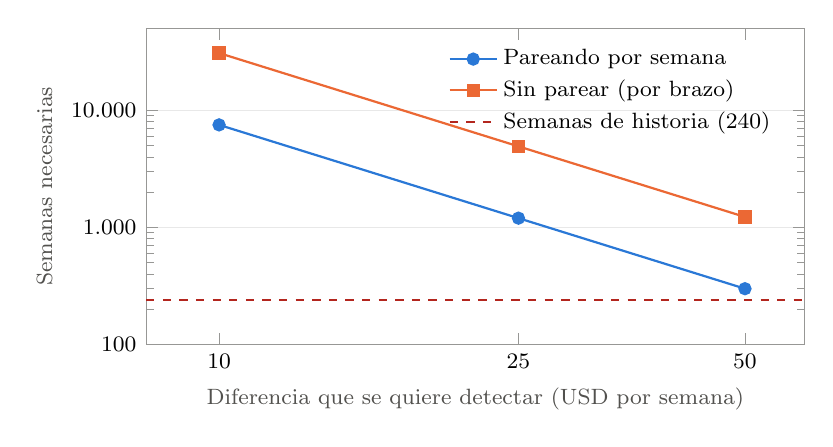
\begin{tikzpicture}
\begin{axis}[estilo, width=0.82\linewidth, height=5.6cm, xmode=log, ymode=log, ymajorgrids,
  xlabel={Diferencia que se quiere detectar (USD por semana)}, ylabel={Semanas necesarias},
  xtick={10,25,50}, xticklabels={10,25,50}, ytick={100,1000,10000}, yticklabels={100,1.000,10.000},
  ymin=100, ymax=50000, xmin=8, xmax=60, legend pos=north east]
\addplot[color=serieA, mark=*, thick] coordinates {(10,7491) (25,1199) (50,300)};
\addplot[color=serieB, mark=square*, thick] coordinates {(10,30693) (25,4911) (50,1228)};
\addplot[color=crojo, dashed, thick] coordinates {(8,240) (60,240)};
\legend{Pareando por semana, Sin parear (por brazo), Semanas de historia (240)}
\end{axis}
\end{tikzpicture}
\caption{Potencia (80~\% de potencia, 5~\% de significancia) en BTCUSD, con la dispersión de la diferencia
Q4$-$estática (309~USD). Los efectos finos exigen reducir la varianza antes que agregar datos.}
\label{fig:potencia}
\end{figure}

\textbf{Qué hacemos.} Toda comparación del plan es pareada (efecto fijo por semana), con intervalos y no solo
promedios, y con métricas que no dependan de una semana extrema (mediana, pérdida en la cola).

\subsection{Las ventanas no prueban a X0 y se llevan el 99,7~\% del cómputo en eso}
\textbf{Qué vimos.} Cada ventana dura 10,0 minutos: 600 segundos buscando soportes desde cero y unos 2~segundos
simulando la semana. La búsqueda se corta por tiempo en el 99,7~\% de las ventanas de BTCUSD y el 92,5~\% de
las de TSLA, y casi nunca converge. El resultado se parece a una \emph{grilla pareja}: el coeficiente de
variación de las distancias entre soportes vecinos es 0,04 (BTCUSD) y 0,03 (TSLA), contra 0,14 a 0,31 en los
soportes de producción (Figura~\ref{fig:cv}). Por ejemplo, en BTCUSD con 170 soportes las distancias
consecutivas son 1.222,5; 1.223,1; \ldots{} USD.

\begin{figure}[H]
\centering
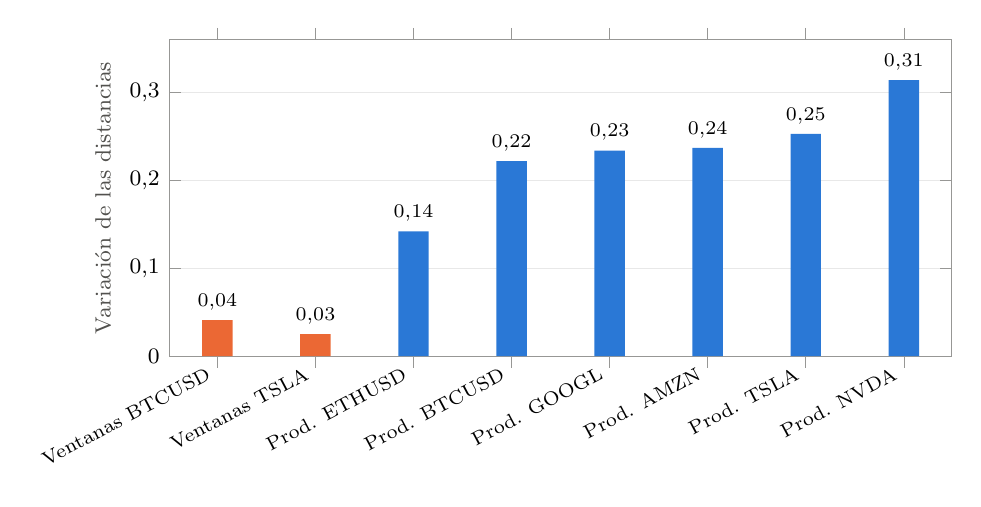
\begin{tikzpicture}
\begin{axis}[estilo, ybar, bar width=11pt, width=0.95\linewidth, height=5.6cm, ymajorgrids, ymin=0, ymax=0.36,
  symbolic x coords={vBTC,vTSLA,pETH,pBTC,pGOOGL,pAMZN,pTSLA,pNVDA}, xtick={vBTC,vTSLA,pETH,pBTC,pGOOGL,pAMZN,pTSLA,pNVDA},
  xticklabels={Ventanas BTCUSD, Ventanas TSLA, Prod. ETHUSD, Prod. BTCUSD, Prod. GOOGL, Prod. AMZN, Prod. TSLA, Prod. NVDA},
  xticklabel style={rotate=28, anchor=east, font=\scriptsize}, ylabel={Variación de las distancias},
  nodes near coords, every node near coord/.append style={font=\scriptsize, color=black},
  nodes near coords={\pgfmathprintnumber[fixed, precision=2]{\pgfplotspointmeta}}, enlarge x limits=0.07]
\addplot[fill=serieB, draw=none, bar shift=0pt] coordinates {(vBTC,0.041) (vTSLA,0.025)};
\addplot[fill=serieA, draw=none, bar shift=0pt] coordinates {(pETH,0.142) (pBTC,0.222) (pGOOGL,0.234) (pAMZN,0.237) (pTSLA,0.253) (pNVDA,0.314)};
\end{axis}
\end{tikzpicture}
\caption{Cuán desiguales son las distancias entre soportes consecutivos (desviación sobre promedio). Los soportes
de las ventanas (naranja) son 5 a 10 veces más parejos que los de producción (azul).}
\label{fig:cv}
\end{figure}

\textbf{Por qué importa.} Todo lo medido hasta hoy se midió sobre una estrategia de grilla cuyo paso lo fija
\code{N}, no sobre la de X0. Además la búsqueda se repite para cada configuración aunque \code{A},
\code{factor\_B} y la pérdida máxima \emph{no la afectan}: con cuenta nueva no hay órdenes abiertas en el punto
de partida, así que los soportes dependen solo de la fecha, de \code{N}, \code{K}, \code{N\_EXP}, \code{LAMBDA},
la semilla y el tiempo. Falta confirmar si la diferencia con producción se debe a una versión anterior de X0
(los archivos de producción son de antes de los saltos del 3 de noviembre), pero 5 a 10 veces parece demasiado.

\textbf{Qué hacemos.} Un \emph{motor de repetición}: se buscan los soportes una vez por semana y valor y se
reutilizan para simular la semana con muchas configuraciones de operación en segundos (§\ref{sec:motor}).

\subsection{La semana con cuenta nueva ve la mitad buena de la estrategia}
\begin{table}[H]
\centering\small
\begin{tabularx}{\linewidth}{lXX}
\toprule
 & Ventanas semanales (BTCUSD) & Cuenta continua con Q4 (2022--2024) \\
\midrule
Trades cerrados ganadores & 98,8~\% (mediana 100~\%) & 72,9~\% \\
Cierres por pérdida máxima & 1~\% & 27~\% (233 de 870; \mn{}7.117~USD en total) \\
Trayectoria de la cuenta & \code{Y} medio $+$68~USD por semana & 3.000 $\rightarrow$ 4.581 $\rightarrow$ \textbf{396} (cinco semanas, mayo 2022) $\rightarrow$ 46~USD \\
\bottomrule
\end{tabularx}
\caption{La semana aislada gana casi siempre; la cuenta continua revela una espiral de pérdidas (previa al tope
de Órdenes Abiertas, que la limita pero no la elimina).}
\end{table}

\textbf{Por qué importa.} La estrategia compra caídas en soportes: gana poco y seguido (unos 3~USD por posición
en BTCUSD) y pierde mucho y rara vez (400~USD en una pérdida máxima, o sea unas 130 ganancias mínimas). En una
semana las pérdidas aparecen solo como flotante, y el dinero \emph{cerrado} se ve suave. El riesgo vive en
\emph{secuencias} de semanas, que una cuenta nueva por ventana no ve. Nadie ha verificado que una cuenta continua
con la configuración estática se acerque a lo que suman sus semanas (+145~USD por semana, mediana 63).
Tampoco hay spread, swap ni comisión en X4 (el spread cuesta alrededor de 9~\% del resultado en BTCUSD y 4~\%
en TSLA; el swap no está medido).

\textbf{Qué hacemos.} El nivel final de decisión es una cuenta continua (tu criterio híbrido, §\ref{sec:embudo}),
con valor de mercado (cerrado más flotante), caída máxima y pérdida en la cola.

\subsection{La calibración de Q4 era circular y el «N dinámico» era un N más bajo}
\textbf{Qué vimos.} Q4 ajusta una curva contra el percentil del propio índice, así que ajusta bien con
cualquier variable: el indicador de fuerza relativa da R$^2=0{,}98$ y el ruido puro 0,998; invertir la hipótesis
de \code{N} da el mismo R$^2$ y el mismo signo «correcto». Además la curva se ajustó con todo el historial
(información futura). Y por construcción el percentil reparte el tiempo parejo entre piso y techo: el \code{N}
dinámico promedia 117--135 soportes contra 180 fijos y está bajo 180 el 95 al 100~\% del tiempo (en acciones, 180 es
el techo del rango).

\textbf{Por qué importa.} Comparar «dinámico contra estático» mide el nivel, no el dinamismo. Un \code{N} fijo
cercano a 125 podría dar lo mismo sin ninguna maquinaria.

\textbf{Qué hacemos.} Todo parámetro dinámico se compara contra un estático \emph{igualado} (fijado en el mismo
promedio) y contra la mejor estática, y su efecto se mide con riesgo.

\subsection{Los parámetros en dólares y las ventanas en velas significan cosas distintas según el activo}
\textbf{Qué vimos.} \code{A}, \code{B} y \code{PERDIDA\_MAX} están en dólares, y X1 los escala por el lote real, así
que equivalen a una \emph{distancia de precio} fija. Medidas en unidades del rango verdadero promedio de una vela
(ATR) y como porcentaje del precio salen muy distintas:

\begin{table}[H]
\centering\small
\begin{tabular}{lrcccc}
\toprule
Activo & Precio mediano & \code{A} en ATR & \code{B} en ATR & Pérdida máx. (\% del precio) & ¿Habría actuado? \\
\midrule
BTCUSD & 77.303 & 0,64 & 0,32 & 25,9~\% & sí \\
ETHUSD & 2.320 & 1,59 & 0,79 & 86,2~\% & sí \\
TSLA & 399 & 0,73 & 0,37 & 50,1~\% & sí \\
GOOGL & 335 & 1,14 & 0,57 & 59,6~\% & \textbf{no} \\
NVDA & 197 & 1,69 & 0,85 & 101,5~\% & \textbf{no} \\
AMZN & 243 & 1,69 & 0,85 & 82,5~\% & \textbf{no} \\
MSFT & 448 & 0,99 & 0,50 & 44,6~\% & por poco \\
\bottomrule
\end{tabular}
\caption{Los valores «estáticos» de \code{config.py} expresados en unidades de mercado (precio mediano de los
últimos 365 días). Además cambian en el tiempo: en NVDA, \code{A} pedía 11,4 ATR en 2022 y 1,7 ATR en 2026.}
\end{table}

Las ventanas del análisis (30~días, 7~días, el suavizado) están definidas en \emph{número de velas} suponiendo
24 por día. En cripto es cierto; en TSLA, NVDA, AMZN y MSFT hay 10 velas con datos por día y en GOOGL 7:
«30 días» son 72 días de mercado (103 en GOOGL).

\textbf{Por qué importa.} El valor «estático» ya se mueve con el precio y en sentido contrario al de la
hipótesis; la pérdida máxima nunca actúa en tres de siete activos; y las conclusiones entre activos están
contaminadas por horizontes distintos.

\textbf{Qué hacemos.} Expresar \code{A} y \code{B} como múltiplos de la volatilidad,
$A_t = k_A\cdot \mathrm{ATR}_t\cdot L_{\min}$ (y lo mismo para \code{B}), \emph{ya es} la hipótesis
«volatilidad alta, \code{A} alto» con un solo número por parámetro. Es el primer peldaño de la escalera
(§\ref{sec:escalera}). Y todas las ventanas pasan a tiempo calendario o días de mercado.

\subsection{El aprendizaje no encontró señal, y hay razones de diseño}
\textbf{Qué vimos.} Con unas 112 ventanas de aprendizaje por valor, los 26 coeficientes C2 no explican el
resultado por sobre el mercado de la semana: R$^2$ con solo los controles de $+0{,}10$ (TSLA) y $+0{,}16$
(BTCUSD); con los 26 coeficientes, $+0{,}004$ y $+0{,}09$; al barajar las filas, $p=0{,}93$ y $0{,}66$.
Las razones de diseño: (1) el \emph{instrumento es débil}, porque el estado del activo, y no el sorteo,
determina entre 57 y 92~\% de lo que valen los parámetros; (2) las derivadas \emph{cambian de signo} (el efecto de
la pendiente depende del lado del punto medio en que esté el índice) y un modelo lineal promedia
efectos opuestos; (3) las pendientes de 8 a 12 vuelven a la curva un interruptor, con el 63~\% de las
ventanas en el 10~\% extremo del rango; (4) el ascenso de gradiente se mueve el 10~\% del rango aunque el
modelo diga «no hay señal»; (5) tras 32 ventanas el sorteo deja de explorar; (6) el signo de cada curva se
impone de antemano.

\textbf{Por qué importa.} No es solo ruido: el diseño mismo (aprender coeficientes de una curva de 4 números por
parámetro, con efectos que dependen del estado) vuelve indetectable cualquier señal real.

\textbf{Qué hacemos.} Aleatorizar \emph{los parámetros mismos} dentro de la misma semana (diseño factorial),
con pocos números por política, y solo después buscar cómo depende el óptimo del estado.

\subsection{Q4 pierde contra la estática todos los años, y lo poco que se mueve es nivel}
\begin{figure}[H]
\centering
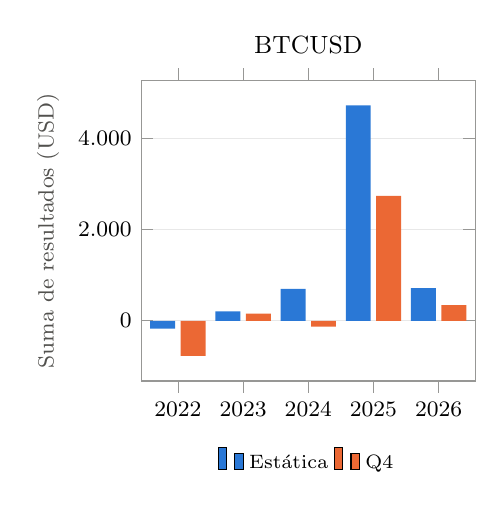
\begin{tikzpicture}
\begin{axis}[estilo, ybar, bar width=9pt, width=0.48\linewidth, height=5.4cm, ymajorgrids, title={BTCUSD},
  title style={font=\small}, symbolic x coords={2022,2023,2024,2025,2026}, xtick=data, ylabel={Suma de resultados (USD)},
  legend style={at={(0.5,-0.2)}, anchor=north, font=\scriptsize, draw=none}, legend columns=2, enlarge x limits=0.14]
\addplot[fill=serieA, draw=none] coordinates {(2022,-174) (2023,207) (2024,697) (2025,4724) (2026,713)};
\addplot[fill=serieB, draw=none] coordinates {(2022,-771) (2023,154) (2024,-126) (2025,2740) (2026,344)};
\legend{Estática, Q4}
\end{axis}
\end{tikzpicture}\hfill
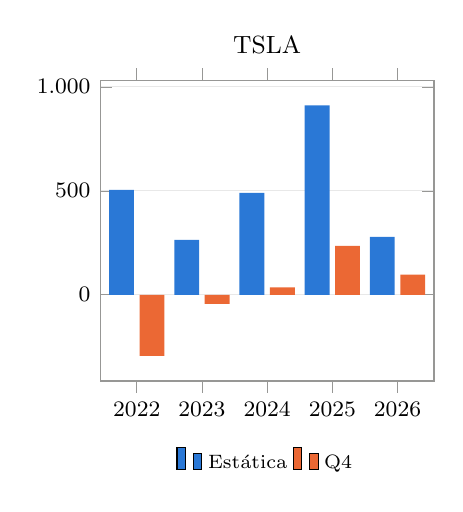
\begin{tikzpicture}
\begin{axis}[estilo, ybar, bar width=9pt, width=0.48\linewidth, height=5.4cm, ymajorgrids, title={TSLA},
  title style={font=\small}, symbolic x coords={2022,2023,2024,2025,2026}, xtick=data,
  legend style={at={(0.5,-0.2)}, anchor=north, font=\scriptsize, draw=none}, legend columns=2, enlarge x limits=0.14]
\addplot[fill=serieA, draw=none] coordinates {(2022,504) (2023,264) (2024,490) (2025,911) (2026,279)};
\addplot[fill=serieB, draw=none] coordinates {(2022,-294) (2023,-44) (2024,36) (2025,235) (2026,97)};
\legend{Estática, Q4}
\end{axis}
\end{tikzpicture}
\caption{Suma del resultado semanal de la estática y de Q4 en las mismas semanas reservadas, por año. La
estática gana en 10 de 10 año-valor.}
\label{fig:anios}
\end{figure}

\textbf{Qué vimos.} En las semanas reservadas, Q4 pierde contra la estática en 33 de 44 (BTCUSD) y 36 de 47 (TSLA),
con $p<0{,}001$. El aprendizaje sí mejora sobre Q4, pero la candidata de BTCUSD queda indistinguible de la
estática (gana 15 de 26, $p=0{,}56$, media \mn{}34~USD) y la de TSLA pierde (4 de 24). El aprendizaje arrancó con
\code{A}=8,8 (Q4) y caminó hacia \code{A}=6 (la estática usa 3): gastó unas 22 horas redescubriendo, a medias, que
\textbf{un \code{A} bajo opera más} y que la semana premia la rotación. Entre los parámetros, lo poco que se ve
está en los de operación y pasa por el \emph{nivel} (cuánto se opera): \code{A} y \code{B} en TSLA, la pérdida
máxima en BTCUSD (probablemente por el cupo de órdenes que fija), y nada en los de búsqueda, que con la
búsqueda cortada hoy \emph{no se pueden medir}.

\textbf{Qué hacemos.} Optimizar primero el nivel de la configuración estática (en unidades de volatilidad y
con piso de \code{A} por debajo de 2~USD, donde hoy está pegado) y solo después preguntar si ese nivel
\emph{cambia con el estado}. Es lo que ya decía el principio del proyecto: «baseline primero».

\subsection{El mecanismo de \code{N} es de riesgo, no de retorno}
Agrupando las velas por el índice de \code{N}, el retorno de los 7 días siguientes no empeora en los estados
adversos (+2,65~\% contra +2,29~\% en los sanos), pero la caída máxima de esos 7 días sí: \mn{}8,6~\% contra
\mn{}5,7~\%, en los siete activos sin excepción. En cripto el retorno a 30 días es peor en estado adverso; en varias
acciones es mejor (TSLA $+$14,4~\% contra \mn{}6,1~\%). Reducir \code{N} cuando el estado es adverso es
\emph{gestión de riesgo}: con «retorno total sin riesgo» se descartaría por la vara equivocada. Los conjuntos
de distinto \code{N} no están anidados (su coincidencia es la del azar), así que cambiar \code{N} en vivo obliga
a reoptimizar y a reemplazar muchas órdenes; la salida es una \emph{máscara}: X0 calcula una vez el conjunto
para \code{N}=200 y X1 opera un subconjunto de tamaño $N_t$. Y \code{A} y \code{N} interactúan: con \code{N}=180
hay 10 a 21 soportes en el 10~\% bajo el precio, espaciados 0,5 a 1,3 ATR, la misma escala que exige \code{A}.

\begin{advertencia}
\textbf{Lo que está bien y se conserva}: la pregunta (parámetros como función del estado), el arnés de ventanas
(importa X0/X1 sin duplicarlos, es reanudable y determinista), la idea de aleatorizar y \emph{parear por semana}
con la misma semilla, el tope de Órdenes Abiertas como control de riesgo real y simple, y la disciplina de
trabajo (hipótesis pre-registradas, causalidad, decisiones con su descarte).
\end{advertencia}

% ════════════════════════════════════════════════════════════════════
\section{Las reglas de la nueva etapa}\label{sec:reglas}

Los hallazgos se resumen en ocho reglas que gobiernan todo lo que sigue. La mayoría ya eran principios del
proyecto que el diseño anterior fue dejando de lado.

\begin{enumerate}[leftmargin=1.6em]
  \item \textbf{Baseline primero}: toda política dinámica debe ganarle a la \emph{mejor} configuración estática, no a la actual.
  \item \textbf{Medir antes de aprender}: el instrumento (rápido, pareado, con ruido conocido) viene antes que cualquier modelo.
  \item \textbf{Mismas semanas, misma semilla}: toda diferencia entre configuraciones es pareada.
  \item \textbf{Lo barato adentro, lo caro una vez}: lo que se repite miles de veces cuesta segundos; las búsquedas de horas se hacen una vez y se reutilizan.
  \item \textbf{Pocos números por política}: una política dinámica tiene a lo más 2 a 4 números y 2 variables pre-registradas con su signo.
  \item \textbf{Un cambio a la vez}: un parámetro (o un grupo de operación) por experimento, y solo se sube de peldaño si el anterior no basta.
  \item \textbf{Toda afirmación lleva intervalo}, control de comparaciones múltiples y un bloque de confirmación que se mira una sola vez.
  \item \textbf{Unidades de mercado}: volatilidad (ATR) y días de mercado, no dólares ni velas, salvo para comparar con lo actual.
\end{enumerate}

\begin{table}[H]
\centering\small
\begin{tabularx}{\linewidth}{lXX}
\toprule
 & Decisión del 22 de noviembre & Consecuencia en el plan \\
\midrule
Objetivo & «Me encantaría la cuenta continua, pero es muy lento; ideal un híbrido» & Embudo de tres niveles: filtro semanal pareado rápido $\rightarrow$ cuenta continua barata $\rightarrow$ examen continuo con X0 real (§\ref{sec:embudo}) \\
Meta & X5 solo vale si hay dinamismo & La mejor estática es el piso a superar; la escalera busca dinamismo en varias formas; si se agota no se cierra X5 solo (§\ref{sec:rescate}) \\
Cómputo & Mac casi dedicado, 30 o más horas por semana & Cabe construir bancos de soportes de calidad de producción y correr BTCUSD y TSLA en paralelo (§\ref{sec:costos}) \\
\bottomrule
\end{tabularx}
\caption{Tus decisiones y cómo las traduce el plan.}
\end{table}

\paragraph{Qué dejamos de hacer desde hoy.} Correr ventanas del esquema anterior (10 minutos cada una, regresión sin señal,
26~\% descartadas por solape); agregar variables a la regresión o pasar a una red neuronal sobre ~120 ventanas;
publicar \code{K}, \code{N\_EXP} y \code{LAMBDA} como dinámicos; leer la demo como evidencia de rendimiento (sirve para la
mecánica); y poner plata real antes de que una configuración pase el examen y la demo.

% ════════════════════════════════════════════════════════════════════
\section{La propuesta en dos piezas: un embudo para medir y una escalera para subir}

\subsection{El embudo de tres niveles (tu criterio híbrido)}\label{sec:embudo}

Tu objetivo tiene dos mitades que se contradicen: la mejor vara es la cuenta continua, pero es lenta; la más
rápida es la semana pareada, pero ve solo la mitad del riesgo. El embudo las encadena: lo rápido descarta mucho,
lo lento confirma poco.

\begin{figure}[H]
\centering
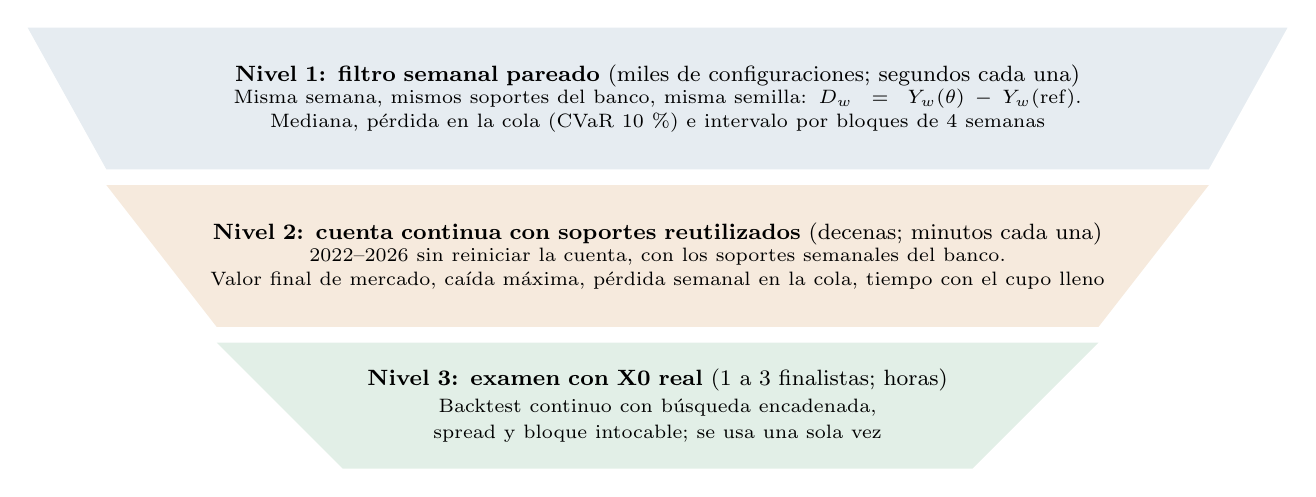
\begin{tikzpicture}[scale=1.0]
\fill[cazul!12] (0,0) -- (16,0) -- (15,-1.8) -- (1.0,-1.8) -- cycle;
\fill[cnaranja!14] (1.0,-2.0) -- (15,-2.0) -- (13.6,-3.8) -- (2.4,-3.8) -- cycle;
\fill[cverde!14] (2.4,-4.0) -- (13.6,-4.0) -- (12.0,-5.6) -- (4.0,-5.6) -- cycle;
\node[align=center, font=\footnotesize, text width=13.2cm] at (8,-0.9) {\textbf{Nivel 1: filtro semanal pareado} (miles de configuraciones; segundos cada una)\\
  \scriptsize Misma semana, mismos soportes del banco, misma semilla: $D_w=Y_w(\theta)-Y_w(\mathrm{ref})$.\\[-1pt]
  \scriptsize Mediana, pérdida en la cola (CVaR 10~\%) e intervalo por bloques de 4 semanas};
\node[align=center, font=\footnotesize, text width=12.8cm] at (8,-2.9) {\textbf{Nivel 2: cuenta continua con soportes reutilizados} (decenas; minutos cada una)\\
  \scriptsize 2022--2026 sin reiniciar la cuenta, con los soportes semanales del banco.\\[-1pt]
  \scriptsize Valor final de mercado, caída máxima, pérdida semanal en la cola, tiempo con el cupo lleno};
\node[align=center, font=\footnotesize, text width=10.4cm] at (8,-4.8) {\textbf{Nivel 3: examen con X0 real} (1 a 3 finalistas; horas)\\
  \scriptsize Backtest continuo con búsqueda encadenada, spread y bloque intocable; se usa una sola vez};
\end{tikzpicture}
\caption{El embudo. El criterio final es el retorno total de la cuenta continua con riesgo acotado; el nivel 1
solo decide quién pasa a verlo.}
\end{figure}

\begin{table}[H]
\centering\small
\begin{tabularx}{\linewidth}{lXXX}
\toprule
 & Nivel 1 & Nivel 2 & Nivel 3 \\
\midrule
Qué mide & ganancia semanal contra la referencia, en pares & valor final de la cuenta continua con riesgo & lo mismo, con X0 real y costos \\
Costo por evaluación & 2 a 4 s & 8 a 16 min por activo & 2 a 3 h por activo \\
Aproximación que acepta & soportes fijos por semana, cuenta nueva & soportes fijos por semana; OA no entran a la FO & ninguna (X4 normal con warm start) \\
Criterio para pasar & intervalo del 90~\% de la media pareada sobre 0; CVaR no peor en más de 10~\% & valor final $\geq$ mejor estática y caída máx. no peor & intervalo sobre 0 en el bloque reservado; sin peor caída \\
\bottomrule
\end{tabularx}
\caption{Los tres niveles. La aproximación del nivel 2 (con soportes precalculados, las órdenes abiertas no entran a la función objetivo como
en X0 real) se valida en 10 semanas contra una corrida con X0 real antes de usarlo.}
\end{table}

Los umbrales numéricos (caída máxima tolerable, cola) te los pido en §\ref{sec:decisiones}. Mi propuesta de
partida, tomada de tus datos: pérdida en la cola (CVaR 10~\%) no peor que la de la estática actual
(\mn{}300~USD por semana en BTCUSD y \mn{}85 en TSLA) y caída máxima de la cuenta continua menor a 40~\%.

\subsection{El motor de repetición y el banco de soportes}\label{sec:motor}

La pieza que vuelve práctico todo lo demás. Una ventana hoy hace dos cosas: \emph{buscar} los soportes
(600~s) y \emph{operar} la semana (2~s). El motor las separa:

\begin{enumerate}[leftmargin=1.6em]
  \item \textbf{Buscar}: para cada semana y valor se busca el conjunto de soportes una vez y se guarda, indexado por
        \emph{los cuatro} parámetros de búsqueda (\code{N}, \code{K}, \code{N\_EXP}, \code{LAMBDA}) y la fecha. Hoy
        existen 627 conjuntos (BTCUSD y TSLA) que sirven de partida.
  \item \textbf{Operar}: con los soportes ya guardados se simula la semana con cualquier combinación de
        \code{A}, \code{factor\_B}, pérdida máxima y tope de OA, con la misma semilla. Cuesta unos 2 a 4 segundos
        (unas 300 veces menos que hoy).
\end{enumerate}

Hay una pregunta previa que decide qué banco construir: ¿los soportes de X0 valen más que una grilla pareja?
Si la respuesta es «no», la estrategia es en el fondo una grilla cuyo paso fija \code{N}, y el banco puede
generarse en segundos; si es «sí», se construye un banco de calidad de producción (búsquedas encadenadas con
warm start, 24 a 40 horas por valor). Esa es la Fase 2 del plan y la primera bifurcación.

\subsection{La escalera del dinamismo}\label{sec:escalera}

Como X5 solo vale si hay dinamismo, el plan no se queda en la estática: la usa como rival y sube por una escalera
de formas cada vez más ricas. Cada peldaño tiene pocos números y debe ganarle al peldaño anterior; si no, no se sube.

\begin{figure}[H]
\centering
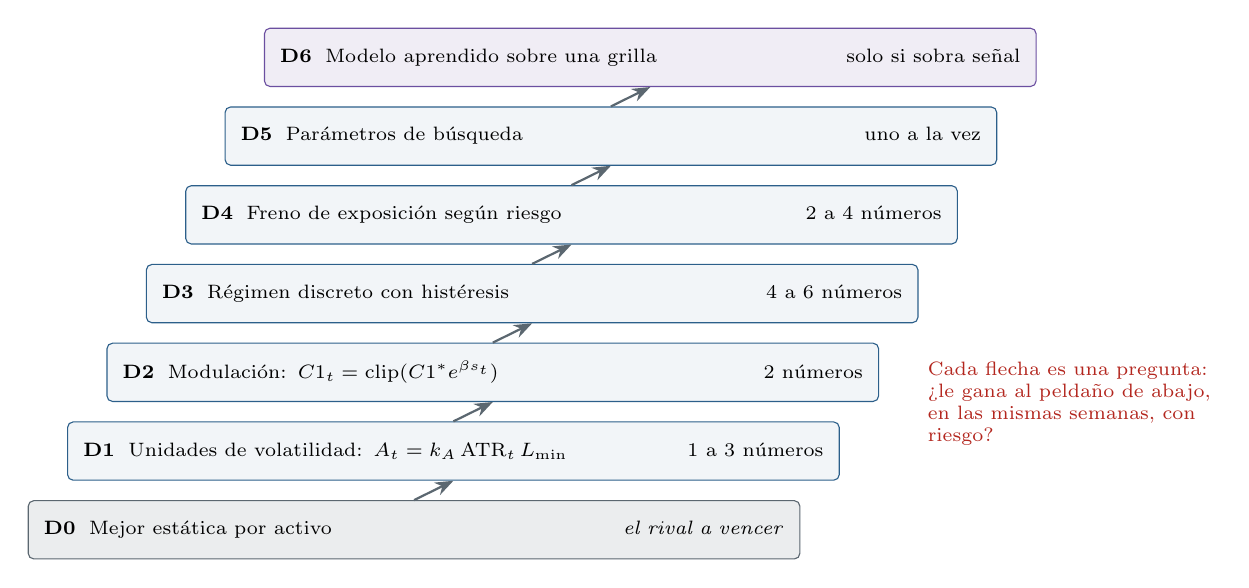
\begin{tikzpicture}[
  p/.style={draw=cazul, fill=cazul!6, rounded corners=2pt, minimum width=9.8cm, text width=9.4cm, minimum height=0.74cm,
            align=left, font=\scriptsize, inner xsep=5pt},
  g/.style={-{Stealth}, color=cgris, thick}]
\node[p, fill=cgris!12, draw=cgris] (d0) at (0,0) {\textbf{D0}\; Mejor estática por activo \hfill \emph{el rival a vencer}};
\node[p] (d1) at (0.5,1.0) {\textbf{D1}\; Unidades de volatilidad: $A_t=k_A\,\mathrm{ATR}_t\,L_{\min}$ \hfill 1 a 3 números};
\node[p] (d2) at (1.0,2.0) {\textbf{D2}\; Modulación: $C1_t=\mathrm{clip}(C1^{*}e^{\beta s_t})$ \hfill 2 números};
\node[p] (d3) at (1.5,3.0) {\textbf{D3}\; Régimen discreto con histéresis \hfill 4 a 6 números};
\node[p] (d4) at (2.0,4.0) {\textbf{D4}\; Freno de exposición según riesgo \hfill 2 a 4 números};
\node[p] (d5) at (2.5,5.0) {\textbf{D5}\; Parámetros de búsqueda \hfill uno a la vez};
\node[p, fill=cmorado!10, draw=cmorado] (d6) at (3.0,6.0) {\textbf{D6}\; Modelo aprendido sobre una grilla \hfill solo si sobra señal};
\foreach \a/\b in {d0/d1,d1/d2,d2/d3,d3/d4,d4/d5,d5/d6}{\draw[g] (\a.north) -- (\b.south);}
\node[font=\scriptsize, color=crojo, anchor=west, text width=3.6cm, align=left] at (6.4,1.6)
  {Cada flecha es una pregunta: ¿le gana al peldaño de abajo, en las mismas semanas, con riesgo?};
\end{tikzpicture}
\caption{La escalera. Se sube solo si el peldaño inferior no alcanza; el modelo aprendido (D6) solo entra si
alguna forma simple mostró que el óptimo cambia con el estado.}
\label{fig:escalera}
\end{figure}

\begin{table}[H]
\centering\small
\begin{tabularx}{\linewidth}{lXXX}
\toprule
Peldaño & Hipótesis & Prueba & Se abandona si \\
\midrule
D1 & El valor «correcto» de \code{A}, \code{B} y pérdida máxima es una cantidad de volatilidad, no de dólares & \code{A}, \code{B}, \code{p} en ATR contra la mejor combinación en dólares, en pares & no le gana a D0 en validación ni en la cuenta continua \\
D2 & El óptimo de un parámetro de operación sube o baja con una variable de estado & contraste $u_w=D_w(\text{alto})-D_w(\text{bajo})$ sobre el estado en $t^*$ (nivel~1) & permutación del máximo $p>0{,}05$ o R$^2$ por bloques $<0{,}05$ \\
D3 & Hay 2 a 3 regímenes con configuración óptima distinta & mejor configuración por régimen contra D0, con histéresis de 24~h & ningún régimen supera a D0 con intervalo sobre 0 \\
D4 & Frenar exposición en estados de riesgo mejora retorno ajustado por riesgo & tope de OA y máscara según drawdown y volatilidad (nivel~2) & no mejora CVaR ni caída máxima sin perder retorno \\
D5 & El nivel de \code{K}, \code{N\_EXP}, \code{LAMBDA} importa y cambia con el régimen & métricas de soporte y banco con 3 niveles por parámetro & sin efecto sobre el resultado: se fijan \\
D6 & Hay interacciones suaves que las formas simples no capturan & GB con restricciones de monotonía (o GAM) sobre unas 12.000 filas & no le gana a la mejor forma simple en validación por bloques \\
\bottomrule
\end{tabularx}
\caption{Qué se supone y cómo se pone a prueba cada peldaño. El orden recomendado de ataque es D1, D4, D2, D3, D5 (más barato y más probable primero).}
\end{table}

\paragraph{Variables de estado.} Se parte de un universo acotado (10 a 20 candidatas, una por grupo con
$|\rho|<0{,}7$) en familias: volatilidad (ATR relativo, razón corta/larga), tendencia (fuerza direccional, retornos de
7/30/90 días, distancia a la media de 200), drawdown (7/30/90 días, distancia al máximo histórico), rango, volumen,
y calendario. Se descartan los fundamentales (sin histórico usable) y el coseno sin centrar. Las ventanas se
definen en tiempo, no en velas. Se pre-registran a lo más dos variables por parámetro, con su signo.

% ════════════════════════════════════════════════════════════════════
\subsection{Un ejemplo con números ficticios}

Para ver cómo encajan el pareo, el banco y la unidad de volatilidad, una semana de BTCUSD (números inventados, solo para
ilustrar). La referencia es la estática actual, \code{A}=3~USD, que con el lote mínimo equivale a una distancia de precio de
300~USD. La política a probar es D1: \code{A} igual a 0,8 veces el ATR (volatilidad) de la hora anterior. En esta semana el ATR
es 500~USD, así que la política exige 400~USD de distancia (un \code{A} de 4~USD). Ambas corren sobre \emph{el mismo conjunto de
soportes del banco, las mismas velas y la misma semilla}:

\begin{center}\small
\begin{tabularx}{0.92\linewidth}{Xrrr}
\toprule
Semana & Referencia $Y_w(\mathrm{ref})$ & Política $Y_w(\theta)$ & Diferencia $D_w$ \\
\midrule
Semana 1 (ATR 500, mercado agitado) & $+120$ & $+150$ & $\mathbf{+30}$ \\
Semana 2 (ATR 250, mercado calmo) & $+40$ & $+55$ & $\mathbf{+15}$ \\
Semana 3 (ATR 700, caída fuerte) & \mn{}310 & \mn{}200 & $\mathbf{+110}$ \\
\bottomrule
\end{tabularx}
\end{center}

Las tres semanas tienen resultados muy distintos entre sí (de $-310$ a $+150$): ese es el ruido del mercado que tapa todo. Pero las
diferencias $D_w$ son todas positivas y mucho más parecidas, porque cada una restó el camino del precio de su semana. Esa es la
ventaja del pareo. Con las 240 semanas se calcula la media y su intervalo; digamos $+12$~USD con intervalo del 90~\% entre
$+3$ y $+21$: la política le gana a la referencia en el nivel~1. Recién entonces pasa al nivel~2, donde se corre la cuenta continua
de 2022 a 2026 con ambas y se compara el valor final, la caída máxima y la peor semana. Si en el nivel~2 la política termina con
más plata pero con una caída máxima mayor, el tope de riesgo decide.

\section{El plan paso a paso}\label{sec:plan}

Siete fases, cada una con su entregable y su criterio. Las fases 2, 3 y 4 terminan en una \textbf{bifurcación}:
lo que se encuentre decide por cuál rama seguir, y eso queda escrito antes de correr.

\begin{figure}[H]
\centering
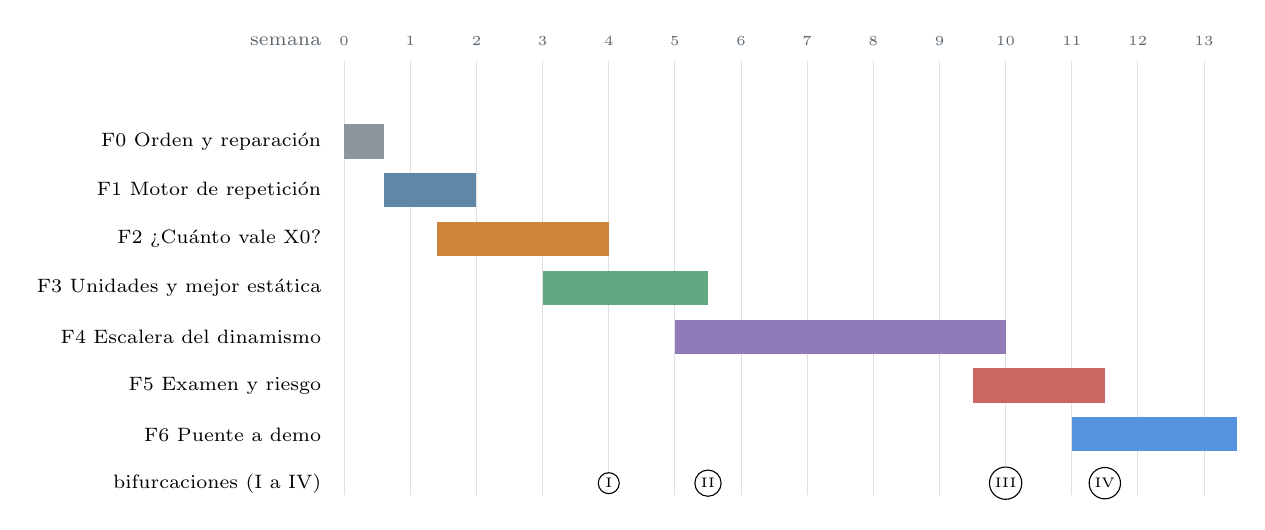
\begin{tikzpicture}[x=0.84cm, y=0.62cm]
\foreach \w in {0,...,13}{\draw[gray!25] (\w,0.3) -- (\w,-8.6); \node[font=\tiny, color=cgris] at (\w,0.7) {\w};}
\node[font=\scriptsize, color=cgris, anchor=east] at (-0.2,0.7) {semana};
\def\bar#1#2#3#4#5{\fill[#5] (#2,-#1) rectangle (#3,-#1-0.7); \node[font=\scriptsize, anchor=east] at (-0.2,-#1-0.35) {#4};}
\bar{1}{0}{0.6}{F0 Orden y reparación}{cgris!70}
\bar{2}{0.6}{2}{F1 Motor de repetición}{cazul!75}
\bar{3}{1.4}{4}{F2 ¿Cuánto vale X0?}{cnaranja!80}
\bar{4}{3}{5.5}{F3 Unidades y mejor estática}{cverde!75}
\bar{5}{5}{10}{F4 Escalera del dinamismo}{cmorado!75}
\bar{6}{9.5}{11.5}{F5 Examen y riesgo}{crojo!70}
\bar{7}{11}{13.5}{F6 Puente a demo}{serieA!80}
\foreach \x/\t in {4/I,5.5/II,10/III,11.5/IV}{\node[draw, circle, inner sep=1.2pt, font=\tiny, fill=white] at (\x,-8.35) {\t};}
\node[font=\scriptsize, anchor=east] at (-0.2,-8.35) {bifurcaciones (I a IV)};
\end{tikzpicture}
\caption{Cronograma con 30 o más horas de cómputo por semana. Las fases se solapan porque el cómputo largo
corre mientras se desarrolla lo siguiente. Los círculos numerados son las bifurcaciones (I a IV).}
\end{figure}

\subsection{Fase 0 — Orden y reparación (días 1 a 4)}\label{sec:f0}
\begin{table}[H]
\centering\small
\begin{tabularx}{\linewidth}{lX}
\toprule
Tarea & Detalle \\
\midrule
0a Respaldo y archivo & Respaldar \code{X5\_otros/} fuera del Mac (lo irrecuperable son los \(\approx\)104~MB de \code{q5/} y los PDF). Copiar a \code{X5/archivo/} las piezas marcadas «rescatar» o «archivar» (§6 de \code{contexto\_x5.md}), con tu visto bueno. \\
0b Diseñar y reparar X4 junto con el motor de X5 & \code{X4\_backtester.py} importa \code{x5\_demo} al inicio (línea 36) y falla. No se repara por separado: primero un diseño conjunto (qué se quita del modo \code{--x5}, qué funciones expone X4 y cómo las llama el motor sin duplicar lógica), que tú apruebas; después se implementa junto con la Fase 1. Se conserva lo que el motor necesita (tope de OA, semillas, tope de tiempo de la búsqueda) y se verifica el modo por versión. \\
0c Residuos & Borrar de \code{config.py} el bloque del macrobrain (líneas 336--441); limpiar comentarios de X0; recortar \code{documentacion.html} y \code{algoritmos.tex} a X4; actualizar \code{vision.md}, \code{CLAUDE.md}. \\
0d Pre-registro & Escribir en \code{decisiones.md}: objetivo híbrido, umbrales de riesgo, bloque intocable (propongo desde el 2026-04-01, unas 28 semanas), criterios de cada fase y la prueba del «candidato nulo». \\
0e Estructura & Scripts en \code{scripts/X5\_*.py}; documentos y pre-registros en \code{X5/}; salidas pesadas en \code{resources/x5/} (fuera de git) y resúmenes pequeños en \code{X5/resultados/}. \\
\bottomrule
\end{tabularx}
\end{table}
\textbf{Criterio de cierre} (se cumple al terminar la Fase 1): \code{import X4\_backtester} funciona y una corrida corta de X4 reproduce un resultado conocido.

\subsection{Fase 1 — El instrumento: motor de repetición (semanas 1 a 2)}
\begin{table}[H]
\centering\small
\begin{tabularx}{\linewidth}{lX}
\toprule
Tarea & Detalle \\
\midrule
1a Separar & Partir \code{ejecutar\_ventana} en \code{buscar\_soportes} y \code{operar\_semana(valor, t*, soportes, config, semilla)}; copiar el estado tras la búsqueda para repetir sin efectos laterales. \\
1b Reproducir & Repetir 20 ventanas con su propia configuración guardada: el resultado debe coincidir con error menor a 0,01~USD. Si no, se investiga el estado compartido antes de seguir. \\
1c Ruido & Dos semillas de la intra-vela en 20 $t^*$ (segundos) y búsqueda repetida con la misma semilla en 10 $t^*$ (unas 2 h): separa el ruido de la simulación, el de la búsqueda y el de la semana. \\
1d Costos & Opción de cobrar spread al llenar (la OE se llena cuando \code{Low}$+$spread$\cdot$punto llega al precio) y apagarla; el swap se estima aparte. \\
1e Registro & Un CSV por valor con la configuración, el resultado, el riesgo y la procedencia de los soportes (extiende el formato de \code{ventanas.csv}). \\
\bottomrule
\end{tabularx}
\end{table}
\textbf{Criterio}: reproducción exacta y costo de 2 a 4~s por semana y configuración. \textbf{Si el ruido de la búsqueda supera la
mitad de la dispersión entre configuraciones}, la Fase 2 pasa a ser lo primero y lo demás espera.

\subsection{Fase 2 — ¿Cuánto vale X0? (semanas 2 a 4) — bifurcación I}
\textbf{Experimento}: en 20 a 40 $t^*$ de BTCUSD y TSLA, buscar soportes «tipo producción» (arranque encadenado
desde la semana anterior, 30 a 60 min de presupuesto, parámetros estáticos) y compararlos con la grilla de las
ventanas en dos cosas: (a) la desigualdad de las distancias frente a la de producción, y (b) el resultado de la
estática con cada uno de los dos, en pares. Cómputo: 10 a 20 h.

\begin{table}[H]
\centering\small
\begin{tabularx}{\linewidth}{lXX}
\toprule
Rama & Si se observa & Qué se hace \\
\midrule
\textbf{I-A} & X0 $\approx$ grilla (diferencia en $Y$ con intervalo que incluye 0) & La estrategia es una grilla cuyo paso fija \code{N}: banco sintético en segundos; \code{N} se explora como paso y se simplifica todo. \\
\textbf{I-B} & X0 $>$ grilla con intervalo sobre 0 & Banco de calidad de producción (24 a 40~h por valor, una vez), indexado por los cuatro parámetros de búsqueda. \\
\textbf{I-C} & depende del activo (p.~ej. cripto sí, acciones no) & Banco de producción solo donde corresponde; grilla en el resto. \\
\bottomrule
\end{tabularx}
\end{table}

\subsection{Fase 3 — Unidades y mejor estática (semanas 3 a 5,5) — bifurcación II}\label{sec:variables}
\begin{enumerate}[leftmargin=1.6em]
  \item \textbf{Unidades}: pasar \code{A}, \code{B} y la pérdida máxima a ATR y todas las variables de estado a tiempo
        (adaptar \code{x5\_alt\_variables.py}: ventanas en días de mercado; quitar fundamentales).
  \item \textbf{Barrido de nivel}: rejilla factorial de operación sobre el banco (\code{A} en USD de 1 a 12 y $k_A$ de 0,3 a 2;
        \code{factor\_B} de 0,3 a 0,7; $p$ de 0,03 a 0,09; \code{N} por máscara de 90, 135 y 180): unas 100 configuraciones
        $\times$ 240 semanas $\times$ 2 s $\approx$ 13 h por valor. Modelo $Y_{wj}=\alpha_w+\text{efecto}_j+\varepsilon$.
        Se elige con 2022-03 a 2024-06, se valida con 2024-07 a 2026-03 y se prefiere una meseta a un pico.
  \item \textbf{Nivel~2} para los 10 a 20 finalistas: cuenta continua. Primera prueba de realidad: la cuenta continua de la
        estática actual; si rinde menos de la mitad de lo que suman sus semanas, el objetivo pasa a ajustado por riesgo desde ya.
  \item \textbf{Etiqueta de cohorte}: tras 7 días, sin OE nuevas, seguir gestionando las OA hasta que cierren o pasen 21 días
        ($Y_{\mathrm{cohorte}}$); si el orden de las configuraciones no cambia (Spearman $>0{,}9$) no hace falta.
\end{enumerate}
\textbf{Entregable}: la mejor estática por activo (con su meseta), la comparación contra la actual y D1 ya probado (su
parte de «unidades»). Costo total: 15 a 25~h por valor.

\begin{table}[H]
\centering\small
\begin{tabularx}{\linewidth}{lXX}
\toprule
Rama & Si se observa & Qué se hace \\
\midrule
\textbf{II-A} & meseta clara y una estática mejor que la actual & Esa estática es la nueva referencia (y una mejora inmediata de producción por sí sola); se sigue a la Fase 4. \\
\textbf{II-B} & paisaje plano (casi nada cambia el resultado) & La operación es insensible: el efecto vive en el riesgo; se prioriza D4 (freno) y la pérdida máxima. \\
\textbf{II-C} & la estática actual ya está en la meseta & La referencia es la actual; sigue la Fase 4 con un listón alto. \\
\bottomrule
\end{tabularx}
\end{table}

\subsection{Fase 4 — La escalera del dinamismo (semanas 4 a 10) — bifurcación III}
Se sube peldaño por peldaño (§\ref{sec:escalera}) con el mismo protocolo, y los datos de la Fase 3 sirven de insumo:
para cada semana y cada parámetro se calcula el contraste $u_w$ (¿esta semana convenía el valor alto o el bajo?, misma
semana, mismos soportes, misma semilla) y se lo explica con el estado causal en $t^*$.

\begin{enumerate}[leftmargin=1.6em]
  \item \textbf{Objetivo limpio}: $u_w$ no contiene el mercado de la semana (es una diferencia pareada).
  \item \textbf{Familias de variables} (10 a 20 candidatas) y validación por \textbf{bloques temporales} con purga (trimestres
        contiguos con una semana de separación).
  \item \textbf{Comparaciones múltiples}: permutación del máximo (barajar $u_w$ en bloques de 4 semanas y recalcular el mejor puntaje
        de todas las candidatas) o control de falsos descubrimientos al 10~\%.
  \item \textbf{Estabilidad}: la variable elegida en más del 70~\% de 500 submuestras por bloques, con el mismo signo en al menos
        4 de 5 años y en BTCUSD y TSLA (o por tipo de activo).
  \item \textbf{Pre-registro}: a lo más 1 o 2 variables por parámetro, con su signo, antes de confirmar en el bloque reservado.
\end{enumerate}

\begin{table}[H]
\centering\small
\begin{tabularx}{\linewidth}{lXX}
\toprule
Rama & Si se observa & Qué se hace \\
\midrule
\textbf{III-A} & heterogeneidad en al menos un parámetro (R$^2$ por bloques $\geq 0{,}05$, $p\leq0{,}05$, mismo signo en ambos activos) & Se construye la forma más simple (D2 o D3), se prueba contra su $\beta=0$ en pares y se pasa al nivel~2. \\
\textbf{III-B} & ninguna en D1 a D3 & Se sube a D4 (freno de exposición según riesgo) y a D5 (búsqueda); si también se agotan, se abre el replanteo (§\ref{sec:rescate}). \\
\textbf{III-C} & solo en un tipo de activo (p.~ej. cripto) & Política por tipo de activo; se vuelve a probar en los otros cinco valores con datos nuevos. \\
\bottomrule
\end{tabularx}
\end{table}

\subsection{Fase 5 — Examen y riesgo (semanas 9,5 a 11,5) — bifurcación IV}
Los finalistas pasan al nivel~3: backtest continuo con X0 real (búsqueda encadenada y warm start, cada semana), spread
encendido y el bloque intocable, \textbf{una sola vez}, registrando cuántas evaluaciones se hicieron.
Criterio de promoción: media pareada contra la \emph{mejor estática} (no contra Q4) con intervalo del 90~\% por bloques
sobre 0, pérdida en la cola no peor en más de 10~\% y cuenta continua sin peor caída máxima. Antes, el \textbf{candidato nulo}
(la estática contra sí misma con otra semilla) debe pasar menos del 10~\% de las veces; hoy la regla «mediana mayor que
cero» deja pasar al azar cerca del 50~\%. Se decide además qué hacer con la pérdida máxima (¿debe actuar?) y con el tope
de Órdenes Abiertas como política de riesgo.

\begin{table}[H]
\centering\small
\begin{tabularx}{\linewidth}{lXX}
\toprule
Rama & Si se observa & Qué se hace \\
\midrule
\textbf{IV-A} & pasa el examen & Se prepara el puente a demo (Fase 6) y se extiende a los otros cinco valores. \\
\textbf{IV-B} & pasa el nivel~2 pero no el 3 & Se mira dónde diverge la aproximación (órdenes abiertas fijas, soportes semanales); se corrige el banco y se repite el examen con una evaluación nueva, no reciclada. \\
\textbf{IV-C} & no pasa y la causa es el costo o el riesgo & Se redefine la política con riesgo explícito (D4) y se vuelve a la Fase 4 con un solo peldaño. \\
\bottomrule
\end{tabularx}
\end{table}

\subsection{Fase 6 — Puente a demo (semanas 11 a 13 y siguientes)}
Solo para lo validado. Se reutiliza el \emph{patrón} del publicador anterior (un archivo por valor escrito de forma atómica,
lectura con respaldo a \code{config.py} si falta o está viejo, registro de eventos en JSON Lines), sin que X0 y X1 dupliquen
lógica, y X1 con el tope de Órdenes Abiertas sobre una cuenta virtual por valor. Antes se cierran las pruebas en Windows
que nunca se hicieron (el historial de órdenes de MT5 no se puede simular en Mac). Con cuenta demo, mínimo 4 semanas
hacia adelante, y plata real solo después de pasar el examen y la demo.

\begin{table}[H]
\centering\small
\begin{tabularx}{\linewidth}{llXX}
\toprule
Bifurcación & Se decide al terminar & Pregunta & Opciones \\
\midrule
I & Fase 2 & ¿X0 vale más que una grilla? & A grilla / B banco producción / C por activo \\
II & Fase 3 & ¿hay una mejor estática y qué tan sensible es el resultado? & A mejora / B plano / C actual ya óptima \\
III & Fase 4 & ¿el óptimo cambia con el estado? & A sí / B no (subir) / C solo en un tipo \\
IV & Fase 5 & ¿el candidato pasa el examen? & A sí / B parcial / C no \\
\bottomrule
\end{tabularx}
\caption{Registro de bifurcaciones. Cada una queda anotada en \code{decisiones.md} \emph{antes} de correr su fase, con el criterio exacto.}
\end{table}

% ════════════════════════════════════════════════════════════════════
\section{Si algo falla: replanteos ya preparados}\label{sec:rescate}

Dijiste que X5 solo vale si hay dinamismo y que si hay que replantear, se replantea. Por eso el plan no cierra X5 en la
estática: si D1 a D5 se agotan sin pasar los criterios, \emph{se abre una conversación} con estas rutas, listas para
ejecutarse:

\begin{enumerate}[leftmargin=1.6em]
  \item \textbf{Amplificar el instrumento}: aleatorizar los parámetros directamente dentro de la misma semana (diseño factorial
        con varios niveles a la vez) y usar ventanas más cortas y más densas (con soportes reutilizados casi no cuestan; arrancar
        cada día en vez de cada semana multiplica las muestras, aunque correlacionadas, y el bootstrap por bloques lo respeta).
  \item \textbf{Juntar activos}: probar un mapa único estado$\rightarrow$política en unidades de ATR para los 7 valores con
        efecto fijo por activo; multiplica por varias veces las semanas efectivas.
  \item \textbf{Cambiar qué es lo dinámico}: separar \code{A\_OE} de \code{A\_TRAILING}; modular el lote con la volatilidad; un
        interruptor de «no operar» en estados malos; o una política de riesgo que mueva el tope de Órdenes Abiertas.
  \item \textbf{Revisar el planteamiento}: quizás el valor está más en gestionar el riesgo de la cuenta completa que en afinar
        cada parámetro por activo.
\end{enumerate}

\begin{clave}
Lo que \emph{no} se hace es cerrar en silencio: si la escalera se agota, el informe de cierre de X5 lo dice con
números y propone cuál de estas rutas seguir, y tú decides.
\end{clave}

% ════════════════════════════════════════════════════════════════════
\section{Cronograma, costos y riesgos}\label{sec:costos}

\begin{table}[H]
\centering\small
\begin{tabularx}{\linewidth}{lc>{\raggedright\arraybackslash}p{3.9cm}X}
\toprule
Fase & Semanas & Cómputo (h) & Producto \\
\midrule
F0 Orden y reparación & 0 a 0,6 & menos de 2 & X4 funciona; archivo y pre-registro \\
F1 Motor de repetición & 0,6 a 2 & 2 a 4 & motor validado y ruido medido \\
F2 ¿Cuánto vale X0? & 1,4 a 4 & 10 a 20 (más 24 a 40 por valor si la rama es I-B) & rama I elegida; banco de soportes \\
F3 Unidades y estática & 3 a 5,5 & 15 a 25 por valor & mejor estática (meseta) \\
F4 Escalera & 5 a 10 & 10 a 40 por valor & política o replanteo \\
F5 Examen y riesgo & 9,5 a 11,5 & 10 a 20 por valor & decisión de promoción \\
F6 Puente a demo & 11 a 13 y siguientes & menos de 5 & demo en Windows; se suman los otros 5 valores \\
\bottomrule
\end{tabularx}
\caption{Presupuesto con tu Mac casi dedicado (30 o más horas por semana). BTCUSD y TSLA corren en paralelo; los otros cinco valores
entran después de actualizar sus datos desde Windows.}
\end{table}

Estimación total para BTCUSD y TSLA: entre 120 y 220 horas de cómputo (de 4 a 7 semanas de tu Mac) repartidas en unas 12 semanas
calendario, que incluyen el desarrollo, la revisión de cada bifurcación y márgenes. Para comparar: el diseño anterior gastaba
unas 46~h por valor en 250 ventanas, una configuración por ventana.

\paragraph{Riesgos principales y qué los controla.}
\begin{itemize}[leftmargin=1.4em]
  \item \textbf{Falsos descubrimientos}: con 240 semanas y 50 variables la «mejor» sale buena por azar. Control: permutación del máximo,
        bloques con purga, estabilidad entre años y activos, pre-registro y un solo uso del bloque intocable.
  \item \textbf{Aproximación del nivel 2}: soportes fijos por semana ignoran que, en X0, las órdenes abiertas entran a la función
        objetivo. Control: validación en 10 semanas contra X0 real y examen final con X0 real.
  \item \textbf{Un solo régimen / un solo episodio}: el año 2025 concentra el 77~\% de lo que gana la estática en BTCUSD, y varias
        decisiones de Q4 se tomaron mirando enero--febrero de 2026. Control: resultados por año y bloque intocable desde abril de 2026.
  \item \textbf{Operativos}: el Mac se suspende (usar \code{caffeinate -i}); OneDrive bloquea archivos en Windows; el resultado de una búsqueda
        con tope de tiempo depende de la carga del equipo. Control: semillas, reanudación y un proceso por valor.
  \item \textbf{Acoplamiento de la cuenta}: el bróker limita las órdenes pendientes, así que en producción los activos compiten. Se mide
        por activo y se revisa como cartera antes de plata real.
\end{itemize}

% ════════════════════════════════════════════════════════════════════
\section{Qué necesito de ti}\label{sec:decisiones}

\begin{table}[H]
\centering\small
\begin{tabularx}{\linewidth}{cXX}
\toprule
\# & Decisión & Mi propuesta \\
\midrule
1 & Revisar el Anexo~A y el \S6 de \code{contexto\_x5.md}: ¿qué se archiva en \code{X5/archivo/}? & el núcleo de ventanas, funciones y variables; el PDF de la revisión de octubre \\
2 & Respaldar \code{X5\_otros/} fuera del Mac antes de moverlo o borrarlo & \code{scripts/} y \code{docs/} ($\approx$18~MB) y \code{q5/} comprimido ($\approx$100~MB) \\
3 & Que X4 se diseñe y repare junto con el motor de X5 (Fases 0b y 1) & sí; diseño conjunto aprobado antes de tocar código \\
4 & Tope de riesgo del objetivo híbrido & CVaR 10~\% no peor que la estática actual; caída máxima de la cuenta continua menor a 40~\% \\
5 & Bloque de confirmación intocable & desde el 2026-04-01 (28 semanas) y la demo hacia adelante \\
6 & ¿Cobrar spread en X4 (afecta todos los backtests)? & sí, con opción de apagarlo \\
7 & ¿Debe actuar la pérdida máxima? (hoy no actúa nunca en GOOGL, NVDA y AMZN) & sí, definida en ATR o como presupuesto de riesgo \\
8 & Orden de ataque de la escalera & D1, D4, D2, D3, D5 \\
9 & Prioridad de activos & BTCUSD y TSLA primero; ETHUSD después; los demás al actualizar sus datos \\
\bottomrule
\end{tabularx}
\caption{Lo que necesito para arrancar la Fase 0. Las decisiones 1 a 3 desbloquean todo; las demás pueden esperar a su fase.}
\end{table}

El plan ya está en \code{todos.md} como una secuencia de ítems con dependencias (el orden de la sección es el orden de ejecución);
el primer pendiente es tu revisión de este informe, y el diseño conjunto de X4 y el motor de X5 es el segundo paso técnico.

% ════════════════════════════════════════════════════════════════════
\appendix
\section{Veredicto por pieza del X5 anterior}

\begin{table}[H]
\centering\footnotesize
\begin{tabularx}{\linewidth}{>{\raggedright\arraybackslash}p{4.4cm}lX}
\toprule
Pieza & Veredicto & Por qué \\
\midrule
\code{x5\_alt\_variables.py} & \textbf{Adaptar} & Causal y probada; pero con ventanas en velas, fundamentales vacíos y 72 columnas. Ventanas en tiempo, 10 a 20 variables, mantener la prueba de causalidad. \\
\code{x5\_alt\_funciones.py} & \textbf{Adaptar} parcial & Rescatar \code{drawdown\_maximo}, \code{redondear\_a\_grilla}, \code{z\_expanding}, \code{suavizar\_ema}, \code{sigmoide\_acotada}; descartar la calibración circular y la jerarquía C1$=f$(C2). \\
\code{config\_smart.py} & \textbf{Adaptar} & Cuenta de 3.000~USD, tope de OA, fechas, semillas y grillas como punto de partida (piso de \code{A} bajo 2~USD). \\
\code{X4\_bckt\_ventanas.py} & \textbf{Adaptar} (núcleo) & \code{ejecutar\_ventana}, selector de $t^*$ por bisección, reserva por hash y registro; fuera Sobol, aprendizaje y compuerta por mediana. \\
\code{X4S\_backtesting\_inteligente.py} & \textbf{Adaptar} parcial & \code{construir\_cfg}, \code{\_buscar\_soportes}, \code{c1\_operacion}, \code{agregar\_fila\_csv}; fuera la vuelta completa. \\
\code{x5\_alt\_aprendizaje.py} & Descartar & RLM + gradiente sobre C2: sin señal. \\
\code{publicador\_c1.py}, \code{params\_din.py}, \code{registro\_din.py} & Descartar ahora; patrón al final & Publicación atómica, respaldo a \code{config.py}, registro JSONL. \\
\code{X5\_macro\_brain.py}, \code{x5\_demo.py}, \code{config\_x5\_default.py} & Descartar & Modelo no validado; \code{x5\_demo} rompe X4. \\
Notebooks Q1--Q4, P1, P2, exploratorio & Descartar & El estándar de reporte ya vive en \code{docs/context/}. \\
Pruebas (96) & Adaptar 18 & Causalidad de variables y de funciones; el resto con su módulo. \\
\code{q5/ventanas/} (627 conjuntos de soportes) y \code{*\_ventanas.csv} & \textbf{Archivar} & Insustituibles: sirven de banco inicial y de línea base de ruido. \\
\code{q5/BTCUSD/} (cuenta continua con Q4) & \textbf{Archivar} & Única evidencia de una cuenta continua. \\
\code{exp\_Q1}--\code{exp\_Q4}, \code{resources/x5/} & Descartar & Regenerables o sin uso. \\
\bottomrule
\end{tabularx}
\caption{Veredicto resumido. El detalle con argumentos y contratos de cada función rescatada está en \code{contexto\_x5.md} \S6.}
\end{table}

\section{Protocolo estadístico y plantilla de pre-registro}

\paragraph{Diferencia pareada.} Para una configuración $\theta$ y una referencia, en cada semana $w$:
$D_w=Y_w(\theta)-Y_w(\mathrm{ref})$, con $Y_w$ el valor de mercado de la cuenta al cierre de la semana menos el capital inicial,
misma fecha de partida, mismos soportes y misma semilla. Se reportan la media, la mediana, la fracción de semanas ganadas y la
pérdida en la cola (CVaR 10~\%, el promedio del 10~\% peor de $Y_w$, redondeado hacia arriba).

\paragraph{Intervalos.} Bootstrap por bloques de 4 semanas (5.000 remuestreos) sobre las $D_w$; el intervalo del 90~\% de la media debe
quedar sobre 0. Prueba de signo y de Wilcoxon como chequeo.

\paragraph{Tamaño de muestra.} Para detectar una diferencia media $\delta$ con 80~\% de potencia y 5~\% de significancia,
$n\approx\bigl((1{,}96+0{,}84)\,\sigma_D/\delta\bigr)^2$ semanas pareadas, con $\sigma_D$ la desviación de la diferencia; con colas
pesadas es optimista (Figura~\ref{fig:potencia}).

\paragraph{Candidato nulo.} Antes de usar un criterio se mide su tasa de falsos positivos corriendo la estática contra sí misma con otra
semilla; debe pasar menos del 10~\% de las veces.

\paragraph{Comparaciones múltiples.} Permutación del máximo (barajar $u_w$ en bloques, recalcular el mejor puntaje entre todas las
candidatas, repetir) o falsos descubrimientos de Benjamini--Hochberg al 10~\%.

\begin{table}[H]
\centering\footnotesize
\begin{tabularx}{\linewidth}{lX}
\toprule
Campo del pre-registro & Contenido \\
\midrule
ID y fecha & p.~ej. \code{X5-D2-A-001}, escrito antes de correr \\
Hipótesis y dirección & «Si la volatilidad relativa sube, el mejor \code{k\_A} sube» (signo $+$) \\
Variable(s) y forma & hasta 2 variables, causales; forma $C1_t=\mathrm{clip}(C1^{*}e^{\beta s_t})$ \\
Datos y bloques & entrenamiento, validación, bloque intocable (fechas exactas) \\
Métrica y umbral & p.~ej. intervalo del 90~\% de la media pareada sobre 0; CVaR no peor en más de 10~\% \\
Control de comparaciones & cuántas candidatas se prueban y con qué corrección \\
Criterio de abandono & qué resultado hace desistir de este peldaño \\
\bottomrule
\end{tabularx}
\caption{Plantilla de pre-registro (una por peldaño de la escalera).}
\end{table}

\section{Glosario mínimo}
\textbf{Parámetros de primera categoría (C1)}: los siete que consumen X0 y X1 (\code{N}, \code{A}, \code{factor\_B}, \code{K},
\code{N\_EXP}, \code{LAMBDA}, pérdida máxima). \textbf{Parámetros de segunda categoría (C2)}: los coeficientes de la curva que los producía (diseño abandonado).
\textbf{Rango verdadero promedio (ATR, \emph{Average True Range})}: promedio de 14 velas del rango verdadero; mide la magnitud
típica del movimiento sin su dirección. \textbf{Orden en Espera (OE)}, \textbf{Orden Abierta (OA)}: orden pendiente en un soporte y
posición ya activa. \textbf{Pérdida condicional en la cola (CVaR, \emph{Conditional Value at Risk})}: promedio del peor 10~\% de resultados.
\textbf{Efecto fijo por semana}: modelar $Y_{wj}=\alpha_w+\text{efecto}_j+\varepsilon$, de modo que $\alpha_w$ absorbe todo lo común a la semana.
\textbf{Meseta}: región amplia de configuraciones con resultado parecido (más confiable que un pico aislado).
\textbf{Gradient Boosting (GB)}, \textbf{Modelo Aditivo Generalizado (GAM)}: modelos que aprenden curvas por tramos; con restricción de monotonía
solo permiten que el efecto suba o baje en la dirección pre-registrada. Más definiciones y las cifras completas: \code{X5/contexto\_x5.md} y \code{X5/X5\_v3.md}.

\end{document}
